\section{Metodologia}
A metodologia adotada neste trabalho envolve a análise comparativa de diferentes linguagens de programação e a biblioteca OpenCV. O processo metodológico foi dividido nas seguintes etapas:

\subsection{Seleção das linguagens e biblioteca}

A biblioteca OpenCV foi escolhida devido à sua ampla adoção na comunidade de visão computacional, suporte a múltiplas linguagens e vasta gama de funcionalidades. As linguagens selecionadas para comparação foram C++, Java e Python, considerando sua popularidade, desempenho e facilidade de uso em projetos de visão computacional.

\subsection{Definição dos critérios de avaliação}

Foram estabelecidos critérios para a avaliação das linguagens e da biblioteca, incluindo desempenho, facilidade de uso e curva de aprendizado, disponibilidade de recursos e comunidade de suporte.

\subsubsection{Facilidade de Uso e Curva de Aprendizado}
Este critério visa avaliar o quão intuitiva e acessível é a utilização da biblioteca OpenCV em cada linguagem de programação. A avaliação foi realizada através de:
\begin{itemize}
    \item Análise da documentação oficial: Verificação da clareza, abrangência e exemplos fornecidos na documentação.
    \item Disponibilidade de tutoriais e recursos online: Pesquisa por tutoriais, cursos e fóruns de discussão relacionados à OpenCV em cada linguagem.
    \item Configuração do ambiente de desenvolvimento: Avaliação da facilidade de instalação e configuração da biblioteca OpenCV em cada linguagem.
    \item Experiência prática: Implementação de tarefas básicas de visão computacional para avaliar a curva de aprendizado.
    \item \textit{Feedback} de desenvolvedores: Coleta de opiniões e experiências de desenvolvedores que utilizaram a OpenCV em cada linguagem.
\end{itemize}

\subsubsection{Desempenho}
O desempenho tem o objetivo de medir a eficiência das linguagens e bibliotecas na execução de tarefas comuns em visão computacional, sob cenários controlados. Para avaliar comparativamente o desempenho das linguagens C++, Java e Python em tarefas de Visão Computacional de tempo real.

\subsection{Testes Qualitativos}

Métrica Qualitativa (Escala Likert): Foi estabelecida uma escala de 1 a 5 (onde 1 = Insuficiente e 5 = Excelente) para classificar três aspectos: (i) clareza da documentação oficial; (ii) disponibilidade de tutoriais/comunidade; e (iii) facilidade de configuração do ambiente (\textit{setup}).

\subsection{Testes Quantitativos de Desempenho}
Os testes quantitativos foram conduzidos para medir o tempo de execução (latência) de um algoritmo clássico de detecção de objetos em imagens estáticas, utilizando a implementação \textit{Haar Cascade} da biblioteca OpenCV. A escolha do algoritmo se deve à sua eficiência, popularidade e presença em aplicações reais de visão computacional, como reconhecimento facial e detecção de placas veiculares.

Todo o código de teste, \textit{scripts} de medição e procedimentos de pré‑processamento foram versionados e disponibilizados no repositório do projeto para garantir reprodutibilidade, \citep{atomOrgGithub}.

Para a realização dos testes, foram seguidos os seguintes procedimentos:

\subsubsection{Definição do Ambiente de Teste}
Ambiente de \textit{Hardware}: Todos os testes foram realizados em uma máquina com as seguintes especificações:
\begin{table}[h]
\centering
\caption{Ambiente de Teste e Versões}
\begin{tabular}{l l}
\hline
\textbf{Linguagem} & \textbf{Versão} \\
\hline
Python & 3.13.5 \\
Java & 21 \\
C++ (GCC) & 10.3.0 \\
\hline
\multicolumn{2}{l}{\textbf{Hardware}} \\
\hline
Processador & AMD Ryzen 5 3600X 6 \textit{Cores} \\
Memória RAM & 32 GB \\
GPU & NVIDIA GeForce RTX 2060\\
S.O. & Windows 10 Pro 64 bits \\
\hline
\textbf{Versão do OpenCV} & \textbf{Método de Instalação} \\
\hline
OpenCV (Python) & 4.11 (\textit{bindings} oficiais cv2) \\
OpenCV (Java/C++) & 4.12 (\textit{Local build}) \\
\label{tab:ambiente_teste}
\end{tabular}
\end{table}

\subsubsection{Seleção do Conjuntos de Dados}
Para compor o corpus de teste, foram utilizados dois conjuntos de dados públicos de referência (\textit{benchmarks}) obtidos via Kaggle, selecionados pela alta variabilidade de cenários “\textit{in-the-wild}”, evitando viés de dados sintéticos ou controlados em laboratório.

Os dados foram organizados em duas fontes para avaliar a robustez dos classificadores:

\begin{description}
    \item[Dataset A — Diverse LPD (License Plate Detection):]
    Fonte: Diverse-LPD training ready (Mikf, Kaggle).\\
    Características: Heterogeneidade geográfica e ambiental, com placas de diversos países (não restritas ao padrão russo dos modelos Haar), ângulos oblíquos, variações de iluminação (sombras, superexposição) e distâncias variadas. Impõe alto desafio de generalização.

    \item[Dataset B — License Plates OCR:]
    Fonte: License Plates 1.2M OCR (TrainingDataPro, Kaggle).\\
    Características: Conjunto volumoso com foco explícito em veículos; utilizou-se amostragem para validar consistência da detecção em imagens de maior resolução e com foco no objeto de interesse.
\end{description}

\subsubsection{Seleção dos Modelos e Parâmetros de Detecção}
Os testes foram executados com dois modelos \textit{Haar Cascade} pré-treinados, selecionados para representar diferentes níveis de complexidade computacional:
\begin{itemize}
    \item \texttt{haarcascade\_license\_plate\_rus\_16stages.xml}\label{mdl:haarcascade_license_plate_rus_16stages}: Modelo com 16 estágios, priorizando velocidade.
    \item \texttt{haarcascade\_russian\_plate\_number.xml}\label{mdl:haarcascade_russian_plate_number}: Modelo focado em detalhes numéricos, com maior densidade de features.
\end{itemize}

Para garantir a isonomia, o método \texttt{detectMultiScale} foi configurado com os mesmos hiperparâmetros nas três implementações:
\begin{itemize}
    \item \textbf{scaleFactor}: 1.1 (redução de 10\% na pirâmide de imagem a cada escala);
    \item \textbf{minNeighbors}: 3 (mínimo de vizinhos para validar uma detecção);
    \item \textbf{minSize}: $30 \times 30$ \textit{pixels}.
\end{itemize}

\subsubsection{Coleta e Tratamento dos Dados de Desempenho}

Para garantir a reprodutibilidade dos testes, foram adotadas múltiplas fontes de consulta, incluindo a documentação oficial das bibliotecas, repositórios de código aberto e artigos técnicos especializados. Nos experimentos práticos, definiram-se dois conjuntos de tarefas-padrão para isolar o desempenho da linguagem:

Os dados brutos de tempo de execução (latência) foram coletados para milhares de iterações. Observou-se que processos em segundo plano do Sistema Operacional e, no caso de linguagens gerenciadas, pausas do \textit{Garbage Collector}, introduziam \textit{outliers} extremos (picos de latência) que não refletiam o desempenho real do algoritmo de visão computacional.

Para mitigar esse ruído e garantir uma comparação justa baseada na eficiência algorítmica, aplicou-se um método robusto de limpeza de dados: Método IQR (Intervalo Interquartil): Foram removidos os registros que excederam o limite superior calculado como $Q3 + 1.5 \times IQR$. Este tratamento eliminou anomalias de sistema (latências > 100ms em processos que levam 5ms), permitindo o uso confiável da Média Aritmética ($\mu$) e do Desvio Padrão ($\sigma$) como métricas centrais de avaliação, juntamente com a Mediana para análise de tendências centrais robustas.

\subsubsection{Implementação e Coleta de Dados}
\label{sec:implementacao_coleta_dados}
Para garantir a isonomia do experimento, foram implementados três algoritmos computacionalmente equivalentes em C++, Java e Python. O \textit{pipeline} de processamento obedece à seguinte sequência lógica:

\begin{enumerate} 
    \item \textbf{Ingestão da Imagem}: carregamento direto da imagem do disco para a memória utilizando a função \texttt{imread} (padrão BGR), sem pré-processamento explícito de cor; 
    \item \textbf{Cronometragem de Precisão}: medição temporal isolada da função \texttt{detectMultiScale}, utilizando relógios monotônicos de alta resolução (nanossegundos) para eliminar a latência de I/O de disco;
    \item \textbf{Pós-processamento}: renderização das \textit{bounding boxes} na imagem original e salvamento em disco para verificação visual; 
    \item \textbf{Persistência}: exportação dos metadados (arquivo, modelo, contagem e tempo em nanossegundos) para arquivos CSV.
\end{enumerate}

Diferentemente de \textit{pipelines} tradicionais, optou-se por passar a matriz de imagem original diretamente ao método de detecção, delegando ao \textit{framework} (OpenCV) qualquer tratamento interno necessário de canais de cor, visando mensurar o tempo total da chamada de API 'como ela é' em uma aplicação final.

O Fluxograma da Figura \ref{fig:fluxograma_pipeline_teste} ilustra o processo completo de cada iteração de teste.

\subsubsection{Referências dos Dados}
\begin{itemize}
    \item Créditos para \href{https://www.kaggle.com/datasets/fxmikf/diverse-lpd-training-ready}{Diverse-LPD training ready} de Mikf em Kaggle.com.
    \item Créditos para \href{https://www.kaggle.com/datasets/trainingdatapro/license-plates-1-209-438-ocr-plates}{License Plates OCR} de TrainingDataPro em Kaggle.com.
\end{itemize}

\begin{figure}[H] 
    \centering
    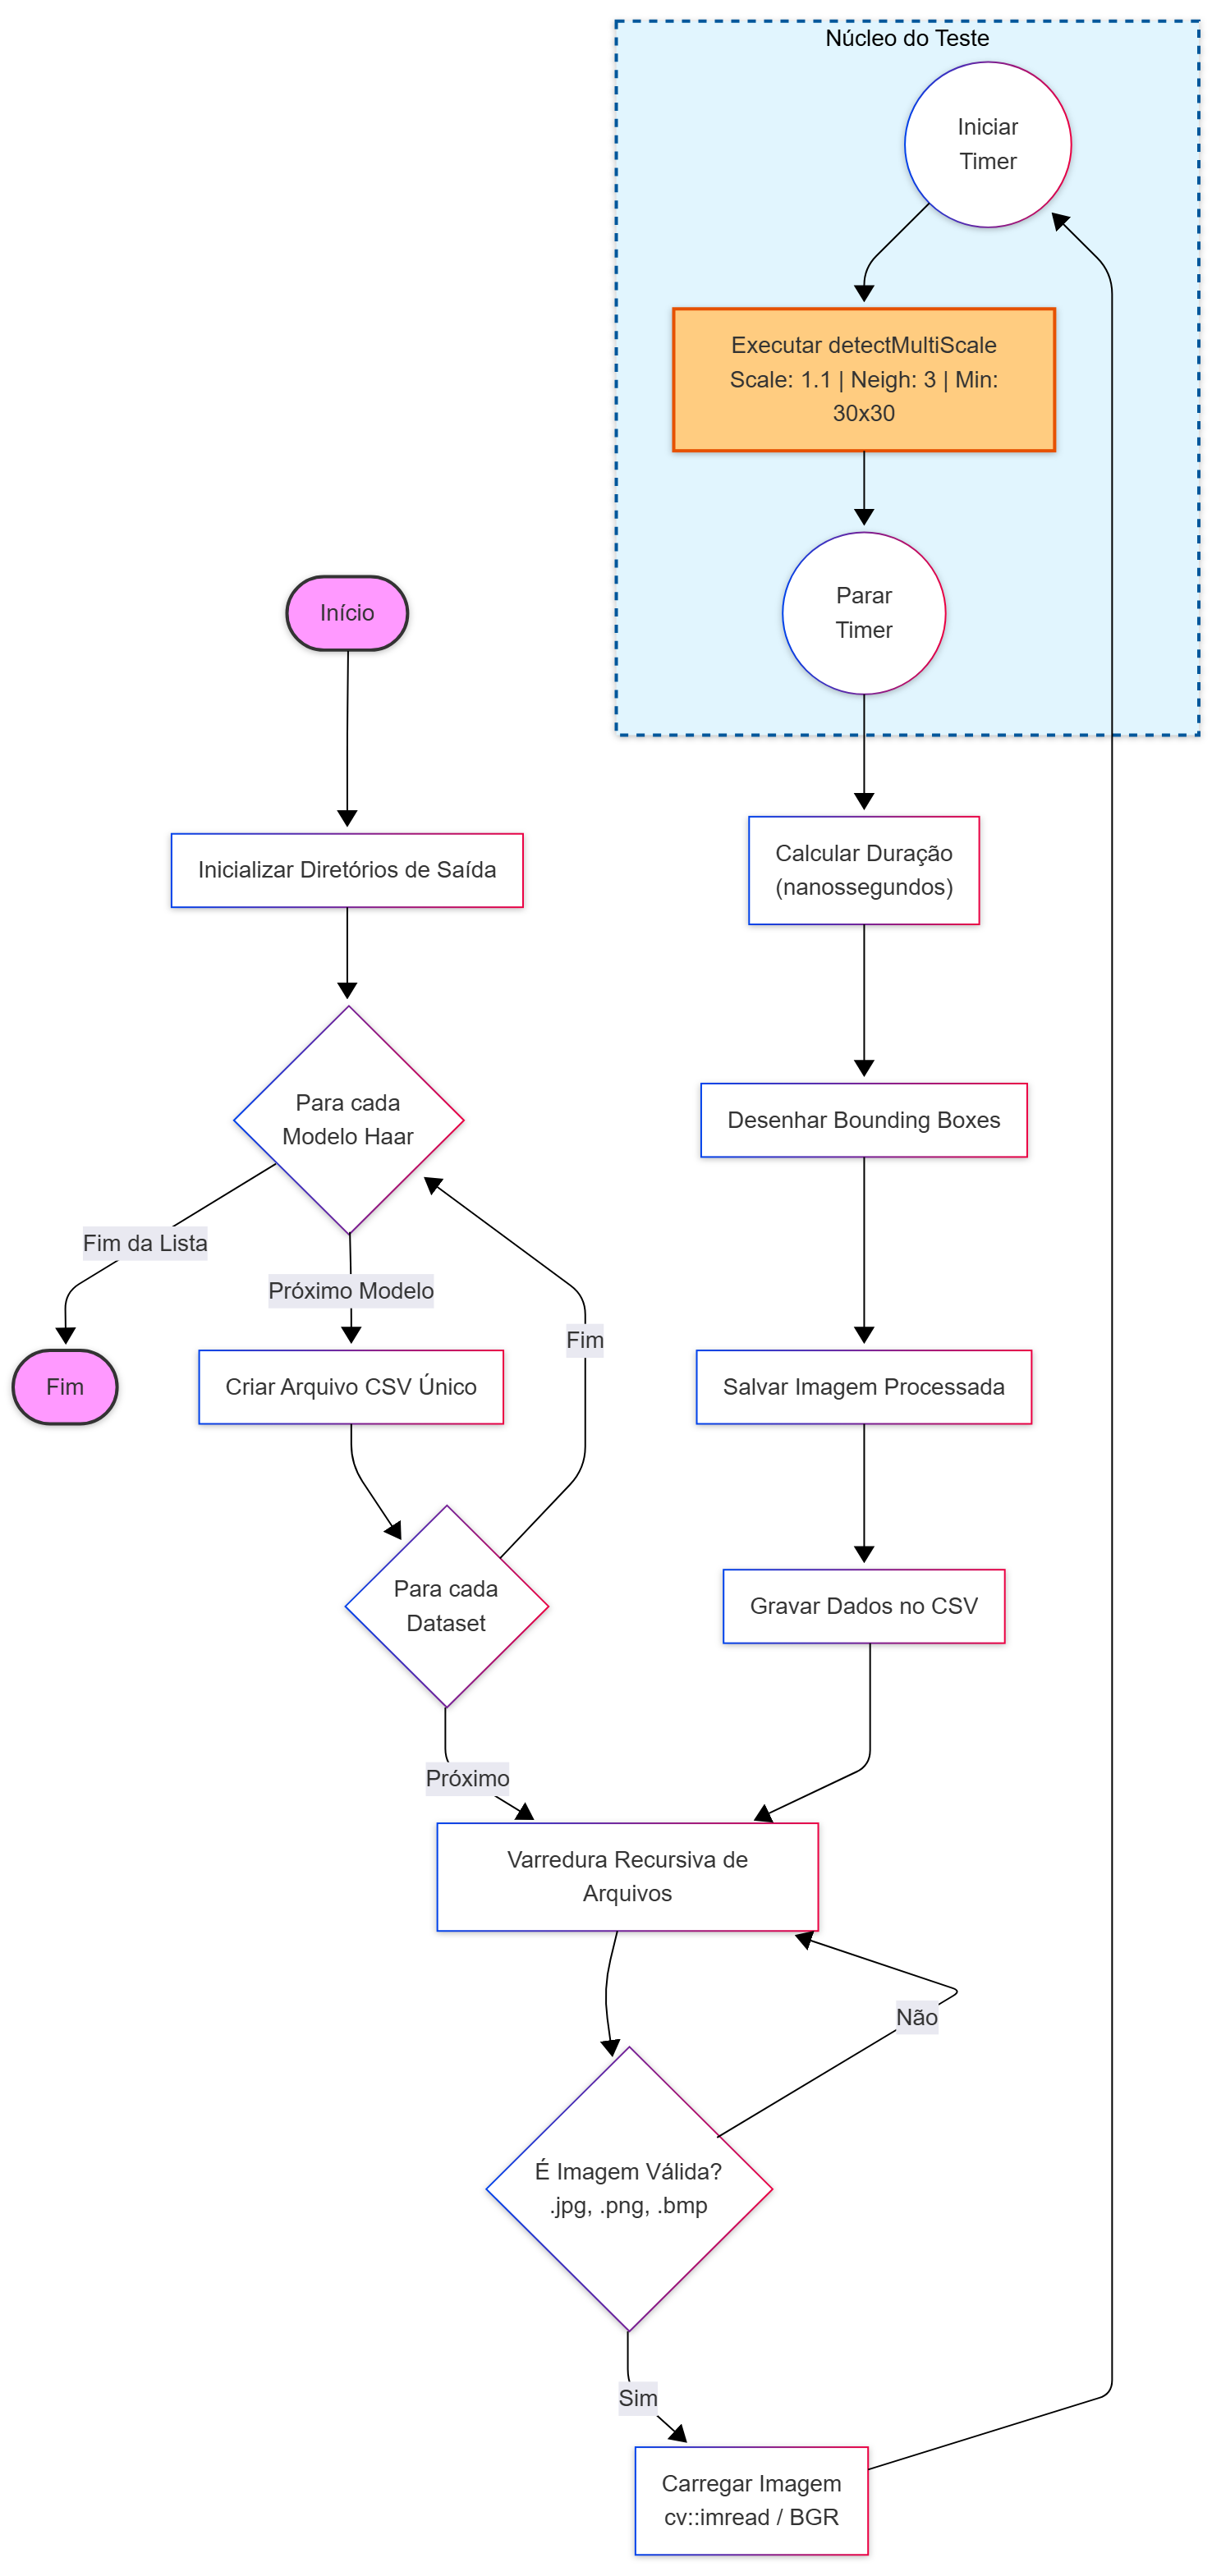
\includegraphics[width=\columnwidth]{images/LicensePlateHaarCascade-FlowDiagram.png}
    \caption{Fluxograma do Pipeline de Teste de Desempenho}
    \label{fig:fluxograma_pipeline_teste}
\end{figure}